\section{Protokół komunikacji bluetooth}
\label{sec:bt-comm}
Robot Dark Explorer komunikuje się z otaczającym go światem przy użyciu
technologii Bluetooth. Zaimplementowany w pierwotnej wersji oprogramowania
robota protokół komunikacji bazuje na ramce składającej się z 8 bitów nagłówka oraz 8 bitów
danych. Za pomocą informacji zawartych w nagłówku robot rozpoznaje
rodzaj akcji którą należy podjąć, natomiast po odczytaniu danych z kolejnego
przesłanego bajtu urządzenie jest w~stanie uruchomić odpowiedni wariant metody
zdefiniowanej w~nagłówku przesłanej ramki. Jeżeli wysłane polecenie wymusza
odesłanie danych zwrotnych są one transmitowane przez robota w~postaci czystego
strumienia bajtów bez żadnych dodatkowych metadanych.

\begin{figure}[h!]
 \centering
 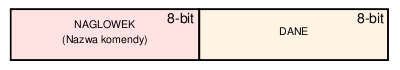
\includegraphics[height=18mm]{../images/ch05/old_req_schema.png}
 \caption{Schemat ramki komunikacyjnej w pierwotnej wersji robota}
 \label{fig:OldCommFrame}
\end{figure}

Zaprezentowane tutaj podejście jest bardzo wydajne i nie ogranicza efektywnej
przepustowości łącza poprzez konieczność przesyłania dodatkowych danych
związanych z obsługą protokołu komunikacji. Nie mniej jednak tego rodzaju
komunikacja wymaga, od programisty tworzącego aplikacje klienckie, głębokiej
znajomości sposobu realizacji poszczególnych poleceń, tak aby mógł on
synchronizować komunikację zarówno pod względem czasowym jak i logicznym. Ma to
szczególne znaczenie w przypadku wykonywania poleceń w sposób sekwencyjny gdzie
aplikacja klienta powinna oczekiwać na zakończenie wykonania poprzedniego
polecenia, jak ma to miejsce np. podczas pobierania obrazu z~kamery. Kolejną
znaczącą niedogodnością jest fakt, iż bardzo często nawet najdrobniejsze zmiany w
oprogramowaniu robota wymuszają wprowadzanie zmian w aplikacji klienta pomimo
tego, że sposób wymiany komunikatów pozostał niezmieniony. Swego rodzaju
kłopotliwym problemem było również interpretowanie odpowiedzi przychodzących z
robota, gdyż aplikacja klienta musiała przechowywać informację na temat rodzaju i
formatu odpowiedzi która została odebrana w wyniku wykonania akcji. Co więcej
dotychczasowy sposób wymiany danych nie gwarantował również mechanizmów
wykrywania i zapobiegania błędom transmisji na poziomie aplikacji.

Zastosowana do wymiany danych technologia bluetooth posiada szereg standardowych
protokołów komunikacyjnych działających w ramach różnych warstw modelu
referencyjnego OSI\footnote{OSI - Open Systems Interconnection - jest to model
referencyjny standaryzujący zasady łączenia systemów otwartych, opisujący w
szczególności strukturę komunikacji sieciowej }. Niestety protokoły dostępne w
warstwie aplikacji ograniczają się jedynie do wymiany danych na temat kontaktów i
synchronizacji danych kalendarzowych, a~co~za~tym idzie nie nadają się do
rozwiązania problemów zdalnego sterowania urządzeń. Pełna~lista protokołów
dostępnych w ramach technologii bluetooth widoczna jest na rysunku
\ref{fig:BtStack}. Niezmiernie ważne jest aby przy projektowaniu schematu
komunikacji w warstwie aplikacji, tak dobrać protokół warstwy niższej aby
realizował on jak najwięcej wymagań postawionych przed systemem komunikacji.

\begin{figure}[h!]
 \centering 
 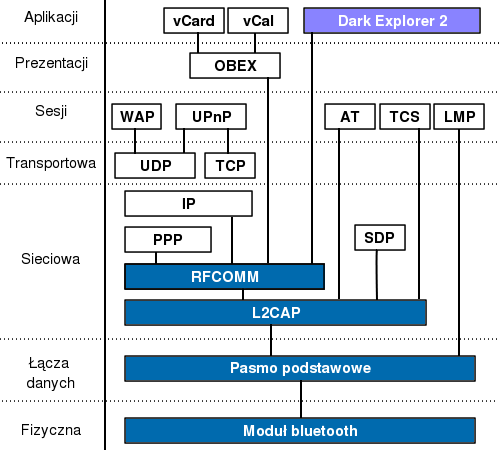
\includegraphics[height=100mm]{../images/ch05/btstack.png}
 \caption{Diagram protokołów bluetooth z podziałem na warstwy}
 \label{fig:BtStack}
\end{figure}

Aby zaadresować wszystkie napotkane w czasie rozwoju robota problemy konieczne
okazało się zaprojektowanie i zaimplementowanie nowego protokołu warstwy
aplikacji który ułatwiłby tworzenie oprogramowania współpracującego z rozbudowaną
wersją robota Dark Explorer. Konieczność taka wynika z faktu iż w warstwie
aplikacji nie istnieją protokoły które możnaby było zaadaptować na potrzeby
sterowania robotem.  Do implementacji protokołu komunikacji wykorzystany został
protokół RFCOMM\footnote{Radio Frequency Communication} gdyż gwarantuje on~nam~korekcję błędów na poziomie pakietów. Wszystkie powiązane z nim protokoły
niższego poziomu zostały oznaczone kolorem na rysunku \ref{fig:BtStack}.

Projekt protokołu komunikacji bazuje na 16 bitowych ramkach bazowych. Każdy przesyłany
komunikat musi posiadać 16 bitowy nagłówek w odpowiednim formacie który pozwoli
na jego poprawne zinterpretowanie i przetworzenie. Komunikaty w niedozwolonym formacie
lub zawierające nieprawidłowe dane będą przez robota ignorowane.

W ramach opracowanego standardu wyróżnić można dwa rodzaje ramek. Do pierwszej grupy
zaliczyć można ramki żądań wysyłane przez urządzenia zewnętrzne w celu zlecenia
robotowi wykonania manewru lub rozpoczęcia kolejnych etapów bardziej złożonej
procedury. Diagram przedstawiający strukturę funkcjonalną ramki żądania widoczny
jest na rysunku \ref{fig:RfcommReqFrame}.

\begin{figure}[h!] 
 \centering
 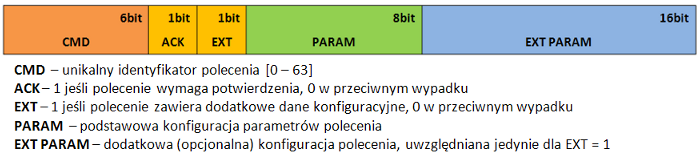
\includegraphics[width=\textwidth]{../images/ch05/req_schema2.png}
 \caption{Schemat funkcjonalny ramki komunikacyjnej z żądaniem}
 \label{fig:RfcommReqFrame}
\end{figure}

Pierwsze 6 bitów zostało zarezerwowane na unikalny identyfikator polecenia które
robot ma wykonać. Pozwala to na zdefiniowanie 64 niezależnych funkcjonalnie
komend w~ramach których, w~wersji podstawowej, możliwe jest uruchomienie 256
niezależnych wariantów polecenia. W przypadku wykorzystania wersji rozszerzonej
nagłówka programista ma do dyspozycji 24 bity które może przeznaczyć na dane
polecenia i identyfikator wariantu komendy w proporcjach odpowiadających
wymaganiom programisty. Kolejny bit nagłówka przeznaczony został na flagę potwierdzenia.
Umieszczenie 1 na wspomnianym bicie spowoduje iż robot po zakończeniu
wykonywania żądania prześle ramkę potwierdzającą ze~statusem wykonania akcji.
Ułatwia to programiście wykonywanie czynności sekwencyjnych takich jak np. wykonanie
zdjęcia za pomocą kamery i przesłanie go~do~aplikacji klienta. Ósmy bit nagłówka
zarezerwowany został na flagę z informacją o użyciu rozszerzonej wersji
nagłówka. Wymuszenie 1 na tym bicie spowoduje, że robot będzie oczekiwał na
dodatkowe 16 bitów danych żądania które mogą zostać wykorzystane do~przesłania
bardziej skomplikowanej konfiguracji wykonania polecenia. Kolejne osiem bitów
stanowi tzw. podstawową konfigurację polecenia, która może służyć jako
identyfikator przy uruchamianiu odpowiedniego wariantu polecenia lub jako nośnik
danych potrzebnych do~zrealizowania przesłanej komendy. W przypadku gdyby
rozmiar bufora konfiguracyjnego nie pozwalał na przechowanie wszystkich
wymaganych danych programista może wykorzystać dodatkowe 2 bajty konfiguracji
rozszerzonej.

Drugi rodzaj ramek stanowią powiadomienia informujące użytkownika o rezultacie 
wykonania przesłanej akcji lub aktualnym stanie robota. Podobnie jak w przypadku
ramki z żądaniem pierwsze 6 bitów zarezerwowane jest na unikalny identyfikator
polecenia dla którego przesyłana jest odpowiedź. Kolejny bit zawiera flagę
informującą o rezultacie zakończenia akcji. Prawidłowe zakończenie wykonania
polecenia sygnalizowane jest ustawieniem zera na wspomnianym bicie. Wystąpienie
błędu podczas realizacji polecenia lub przesłanie komendy w nieprawidłowym
formacie spowoduje ustawienie 1 na bicie STATE. W przypadku gdy ilość
danych do przesłania przekracza maksymalny dopuszczalny rozmiar
pojedynczej ramki możliwe jest podzielenie danych na fragmenty i przesłanie ich
za pomocą sekwencji komunikatów. Koniec sekwencji sygnalizowany jest za pomocą
bitu EOT\footnote{End of Transmission}. Dostępność tego rodzaju trybu pozwala
na szybką transmisję większych ilości danych bez konieczności wysyłania żądań dla poszczególnych fragmentów.

\begin{figure}[h!] 
 \centering
 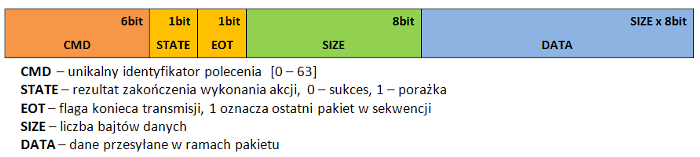
\includegraphics[width=\textwidth]{../images/ch05/resp_schema2.png}
 \caption{Schemat funkcjonalny ramki komunikacyjnej z odpowiedzią}
 \label{fig:RfcommRespFrame}
\end{figure}

Kolejne 8 bitów nagłówka odpowiedzi stanowi informacja o ilości bajtów
przesyłanych w sekcji danych ramki. Ogranicza to maksymalny rozmiar ramki przez
co transmisja danych nie powoduje licznych retransmisji które bardzo często
pojawiają się w przypadku transmisji większych ilości danych. Informacja o
szerokości pola danych ramki może również służyć jako suma kontrolna pozwalająca
na sprawdzenie czy wszystkie zadeklarowane dane zostały prawidłowo odebrane.
Pozwala to programiście tworzącemu oprogramowanie klienta na monitorowanie
transmisji i ewentualne reagowanie w przypadku pojawiania się problemów z
jej płynnością.

% \begin{figure}[h!]
%  \centering
%  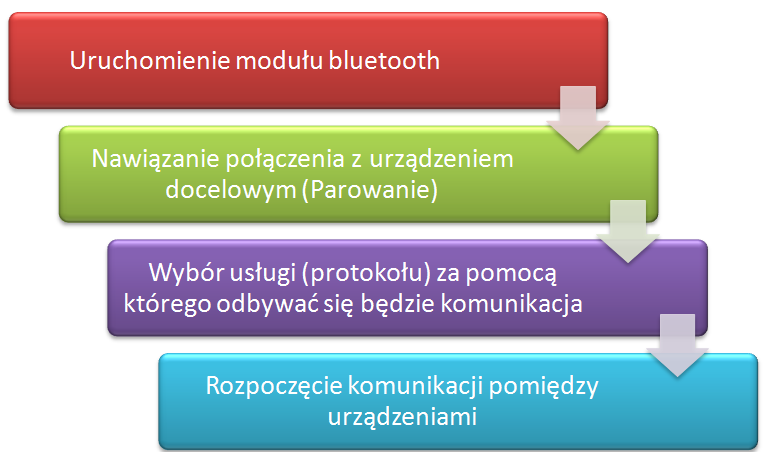
\includegraphics[height=60mm]{../images/ch05/bt_conn_stages.png}
%  \caption{Etapy nawiązywania połączenia bluetooth}
%  \label{fig:BtConnStages}
% \end{figure} 